% !TEX TS-program = pdflatex
% !TEX encoding = UTF-8 Unicode

% This is a simple template for a LaTeX document using the "article" class.
% See "book", "report", "letter" for other types of document.

\documentclass[11pt,twocolumn]{article} % use larger type; default would be 10pt

\usepackage[utf8]{inputenc} % set input encoding (not needed with XeLaTeX)

%%% Examples of Article customizations
% These packages are optional, depending whether you want the features they provide.
% See the LaTeX Companion or other references for full information.

%%% PAGE DIMENSIONS
\usepackage{geometry} % to change the page dimensions
\geometry{a4paper} % or letterpaper (US) or a5paper or....
% \geometry{margin=2in} % for example, change the margins to 2 inches all round
% \geometry{landscape} % set up the page for landscape
%   read geometry.pdf for detailed page layout information

\usepackage{graphicx} % support the \includegraphics command and options
\usepackage{mathtools}
\usepackage{amsmath} % need this stuff for curly brackets
% \usepackage[parfill]{parskip} % Activate to begin paragraphs with an empty line rather than an indent

%%% PACKAGES
\usepackage{booktabs} % for much better looking tables
\usepackage{array} % for better arrays (eg matrices) in maths
\usepackage{paralist} % very flexible & customisable lists (eg. enumerate/itemize, etc.)
\usepackage{verbatim} % adds environment for commenting out blocks of text & for better verbatim
\usepackage{subfig} % make it possible to include more than one captioned figure/table in a single float
\usepackage{authblk}
\usepackage{pdfpages}
\usepackage{wrapfig}
\usepackage{hyperref}
% These packages are all incorporated in the memoir class to one degree or another...

%%% HEADERS & FOOTERS
\usepackage{fancyhdr} % This should be set AFTER setting up the page geometry
\pagestyle{fancy} % options: empty , plain , fancy
\renewcommand{\headrulewidth}{0pt} % customise the layout...
\lhead{}\chead{}\rhead{}
\lfoot{}\cfoot{\thepage}\rfoot{}

%%% SECTION TITLE APPEARANCE
\usepackage{sectsty}
\allsectionsfont{\sffamily\mdseries\upshape} % (See the fntguide.pdf for font help)
% (This matches ConTeXt defaults)

%%% ToC (table of contents) APPEARANCE
\usepackage[nottoc,notlof,notlot]{tocbibind} % Put the bibliography in the ToC
\usepackage[titles,subfigure]{tocloft} % Alter the style of the Table of Contents
\renewcommand{\cftsecfont}{\rmfamily\mdseries\upshape}
\renewcommand{\cftsecpagefont}{\rmfamily\mdseries\upshape} % No bold!

%%% END Article customizations

\title{Software Engineering For Industry \\ AcmeTelecom - Report}
\author[1]{Dan Demeter\thanks{dan.demeter10@imperial.ac.uk}}
\author[1]{Dan Octavian\thanks{dan.octavian10@imperial.ac.uk}}
\author[1]{Razvan Rosie\thanks{razvan.rosie10@imperial.ac.uk}}
\author[1]{Marius Telespan\thanks{marius.telespan10@imperial.ac.uk}}
\affil[1]{Department of Computing, Imperial College London}

\begin{document}
\maketitle

\begin{abstract}
This report describes the implementation of a solution for the problem of improving user bill calculation in a telecommunication company. 
We present a new way of organising the source code in a modular design fashion, in order to improve the process of calculating user bills. Our solution makes use of the best software engineering practices, includes unit and acceptance tests.

Additionally, we have extended the initial solution by providing source code runnable on $Amazon$ $Web$ $Services$ $Elastic$ $Map$ $Reduce$ in order to deal with large sets of customers.
\newline

{\bf Keywords}: acceptance testing, unit testing, design patterns, code refactoring.
\end{abstract}


\section{Introduction}
AcmeTelecom is a telecomommunication company which is currently running calculating the pricing and billing calculations
for all of Acme's mobile phone customers in the following way: if a customer begins a call during the peak time, and the call 
continues in off-peak period, then the whole call is billed at the the peak rate. Similarly, if a customer the call starts in 
the off-peak periodand finish in the peak time, the whole call is billed as being a peak time call. Any call that overlaps the 
peak time period is charged as a peak call.


Our main task was to refactorize the code, making sure that the billing system is fair. In order to make sure that our changes works,
we added acceptance and unit tests covering the existing code.

This report is organised in the following way: {\bf Section 2} presents our implementation of the main feature of the program, which
allows to fairly compute the billings. {\bf Section 3} presents the way that the code was refactorized. 
{\bf Section 4} includes the addition features that were added. 
The fifth section gives an overview of the testing methodologies that were used durin the project, together with the testing tools.
{\bf Section 6} discusses some design decisions that we have taken.
The last part of the report offers our concluding remarks and potential improvements for the code.

\section{ACME Telecom v2}

\subsection{The Improved Cost Calculator}

The given implementation for calculating the call costs, was not taking correctly into consideration 
the $starting$ and $end$ times for a call. As a results, calls which were taking place during both $off$-$peak$ and 
$on$-$peak$ times were being charged for the entire duration with the $on$-$peak$ tariff. For example, for an $on$-$peak$
period of $7:00$ - $18:59$, a call from $20:30$ until $21:30$ would be correctly charged for $60$ minutes $\ast$
$off$-$peak$ tariff, but a call from  $18:30$ until $19:30$ would be charged incorrectly $60$ minutes $\ast$ \textbf{on-peak},
instead of $30$ minutes $\ast$ \textbf{on-peak} $+$ 30 minutes $\ast$ \textbf{off-peak}.

Our code implementation solves this problem, and the algorithm can be described as follows. All $notations$ represented by capital letters 
are $DateTime$ (Joda library) instances:
\begin{enumerate}
\item{For the start call ($START$), find the next ($higher$) peak/offpeak time delimiter ( $7:00$ or $19:00$ ) and save it as $T_1$.}

\item{For the end call ($END$), find the previous ($lower$) peak/offpeak time delimiter ( $7:00$ or $19:00$ ) and save it as $T_2$.}

\item{Compute the seconds between $START$ and $T1$ (reffered as $C_1$) and between $END$ and $T_2$ (reffered as $C_2$).}


\end{enumerate}

The case when $T_1 > T_2$ means that $START$ and $END$ times are in the same peak or off-peak period. Trivially, we compute the 
cost for the call as ($END$ - $START$) $\ast$ ($on$-$peak$ OR $off$-$peak$) tariff. The tariff type can be easily found. 

In the other cases when, $T_1 \leq T_2$, $START$ and $END$ may be in different zones. Therefore, we calculate how many $12$ hours intervals are between $T_1$ and $T_2$.
If that number is even,  we know that $1/2$ of that time the call should be 
charged with the $off$-$peak$ tariff, and the other $1/2$ time should be charged with the $on$-$peak$ time. 
In case that number is odd, then we identify the one extra period (depending if the call started in $on$-$peak$ or $off$-$peak$) and which tariff should be applied to it.

In the end, the final cost is the total cost for the $12$ hours periods $+$ (the cost between $START$ and $T_1$ ($C_1$)) $+$ (the cost between $T_2$ and $END$ ($C_2$). 
Again, for $C_1$ and $C_2$ we can easily identify what tariff we need to use ($peak$ or $off$-$peak$ one).

\subsection{Calls Longer than 24 Hours}

Due to our improved formula for computing the correct and fair cost, we have removed the initial problem 
of calls longer than 24 hours. Our formula takes into consideration any length of time between the calls and 
with the help of our algorithm we can compute the exact cost in a 


\subsection{Joda}
Also, JodaTime helped us a lot in order to manage all the complexity for handling periods of time,
translating the a date into milliseconds and subtracting 2 different Dates. 

\subsection{Printer}
In terms of generating the status of the bills for the customers, the system was directing its results to the Standard Output pipe. 
Unfortunately, the only output interface (HtmlPrinter) was generating HTML tables which were not following the W3C standards. 
Because we have decided to make our system as reliable as possible, we had to take into consideration different set-ups where our system would be running. 
For example, it could run on a server without any output attached (headless server), or for debugging purposes, 
the billing output should be easily read and p arsed from the terminal. 
By using the abstract factory design pattern, we have restructured our Output Interface as an abstract Class, 
having different classes extend it. These classes will be actual printing and formatting the results in a way suitable for the environment.
The current classes we have implemented or changed in the system are: HTMLPrinter and ConsolePrinter. HTMLPrinter is the initial implementation 
of printing the results in an HTML format. We have decided \textbf{not} to change it, because some other legacy software might be parsing the
HTML file generated by our system. This is a major risk, because we can't control what other software interacts with the current one.

Instead, for 100\% legacy compatibility, we have decided to add new Classes extending the Output Interface. 
The first one we have added is the ConsolePrinter class that is used to print the BillingSystem output in a readable format used for debugging.
This is what we have used to test our product, integrating the ConsolePrinter with the Tests we ran. Also, because mostly all new systems will be used 
part of a bigger architecture, we have decided to implement an API interface, used by our system to export its data to other systems. 




\section{Refactoring the code}

\subsection{Package Organisation}
One of the very first tasks was to reorganise the existing source code in a new way.
This was because the existing code was not modular enough. It had classes with too many responsabilities (ex: BillingSystem),
it mixed different aspects of the program in the same methods (ex. bill computation logic and bill html representation) and other aspects.
These things made testing hard (many classes were not unittestable at all), understanding the code difficult and ultimately,
difficult to maintain and extend the codebase.

The major assumption we made is that the interface of billing system remains mostly unchanged. The only modification we made is to add 
a time parameter to the event logging methods, in order to make the system testable and not time dependant.

\subsection{Code restructuring}
We restructured the code in terms of layers of functionality and thinking in terms I/O and method purity.
The functionality of the Billing system includes the following:
\begin{enumerate}
 \item{logging call events}
 \item{computing bills given the information in customer and tarrif databases}
 \item{output pretty-printed bills}
\end{enumerate}
Given this, we maintained BillingSystem as the root class of the system and delegated the above functionality to other classes whose
instances are injected into the BillingSystem instance.

Thus, the logging of events and the log reading in represented through the CallLog interface. Currently, this is implemented using an array.
The flexibility of the interface allows us to use another type of storage (filesystem, database, cloud storage). Note how the use of an iterator
when reading through the logs works with large amounts of data since they are not loaded all in a list and returned. Furthermore, using an iterator allows
for lazy loading as well (ex.: reading 100 log entries at a time from a database instead of all 1 million).

Bill generation logic is encompassed in the BillingJob class. An important thing to note is how this class was written: its 2 methods, aggregateCalls
and createBill are the equivalent of the map and reduce functions respectively of a map reduce job. They can actually be reused to write a map-reduce
class, but they need to be wrapped by methods conforming to the Hadoop API. The reason behind this is to be able to handle large amounts of data
if that is the case in the future. 

The pretty-printing in html format is achieved through the BillPrinter interface (allowing for other types of printing modes to be plugged in).
The current implementation, HTMLBillPrinter has been rewritten to make use of a templating library, Apache Velocity, The reason for this is to make
the representation more easily changeable and to minimize the code. Given the use of a template, even a non-programmer (a designer) can make changes 
without having knowledge of Java.

For the whole code, whe thought in terms of the priciple of purity, side-effects, I/O and testability although more as an inspiration since the
Java type system does not offer support for the above in the way the Haskell language does. Thus, we identified parts of the code which are
"pure" (ex. createBill) and made these methods stateless and dependant only on their parameters, since essentially they are just functions
that take an input and provide an output. This made achieving corectness and testing a lot easier. Obviously, side-effects cannot be avoided in Java,
but by separating database connections, reading the current time from actual processing of data we have many more guarantees about correctness.

\subsection{Removing the cyclic dependencies}
A cyclic dependecy was by the inner class $LineItem$, which was placed inside the $BillingSystem.java$.
The $LineItem$ was used to store customer's phone calls in a data structure.In order to remove the cyclic dependecy, we attached the
data contained by LineItem to the Call object.

The newly refactored code has no cyclic dependencies.

\section{Extra Work}
\subsection{Elastic Map Reduce}
\emph{Elastic MapReduce} is an Amazon-based programming model used for processing very large data sets, 
having its behavior inspired from the functional programming functions $map$ and $reduce$. 
The overall process can be described in the following ways: the input is firstly split in such that it becomes parallelization; 
after this step is performed, each resulting chunk is split again and mapped in a specific category; 
finally, a reduction step is used to eliminate the duplicates in every category and concatenates the results. 
In time, when the application will be required to scale, and the number of customers for $AcmeTelecom$ will be very large, $EMR$ can be extremely 
helpful when computing the costs for conversations and generating the bills as fast as possible. The $EMR$ should be adequate for any 
scalability problems ACME Telecom might face in the future.
\begin{figure}[ht]
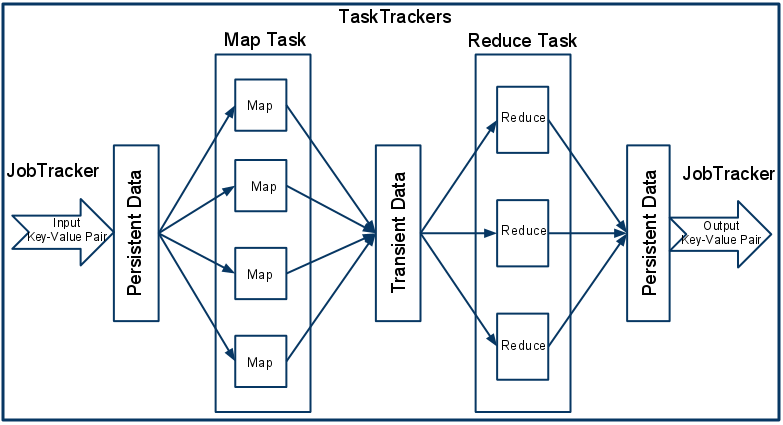
\includegraphics[scale=0.25]{hadoop.png}
\caption{Hadoop \cite{hadoop}}
\end{figure}

\subsection{Speed improvement}

In order to improve the run speed of our system, we have developed our algirhtm to run in \Theta(n)
, where n is the length of the calls for each customer. We assert the fact that for each call,
the \textit{start} and \textit{end} times are chronologically ordered ( the \textit{end} call is \textbf{never}
before the \textit{start} call). Based on our assumption, we can then calculate in \Theta(1), for each call,
what is the total cost associated. 

\subsection{Source code validation}
Another important aspect of software engineering is source code validation. Besides the
aforementioned high level dependency analysis, it is probably worth using tools like Lint4J
and CodePro AnalytiX to audit code, produce metrics, such as Afferent/Efferent Couplings, to measure code quality, and find similar/dead code to identify and remove redundancy, hence streamlining the codebase, in preparation for deployment to target environment.


\subsection{Documentation}
On top of the builtin javadoc tool, the JAutodoc tool was used to generate Java documentation of typical classes like the model CustomerBill for completeness.
Subsequently, additional configuration enabled styling of the resulting generated Javadocs

\subsection{New Output Interface}
As we have descibed before, we have added several Output Interfaces,....

\section{Testing}
Any new software that is developed has the potential to act in a different way other that it was designed in the beginning. So testing is essential for any new piece of software.
In our approach we followed a Test Driven Development (TDD) in order to make sure our system is developed as we intend it to work. 

For this we came up with guides for implementation of the program logic and we made sure the original design contract was implemented successfully when all these tests passed.            
Because of the number of tests, we decided to split tests into two packages: one for Unit Testing and one for Acceptance Testing.


\subsection{Unit Testing}
Unit tests can be found in the package com.acmetelecom.tests.unit. Their primary purpose is to test components individually in isolation. Therefore Mockito\cite{mockito} framework has been used in order to help mock objects for the tests.

In order to asses our test coverage we have used EMMA tool which produces a raport describing classes, methods, blocks and lines tested. A diagram of this can be seen below:

Since our initial coverage was not good enough we have some automatic test generator after in order to cover some of the tests we omit: initialisation of classes, methods calling with null arguments, etc. 
CodPro AnalytiX\cite{codePro}  is an automatic unit test generator tool that helped us to make sure we have a very good test coverage and also to spot any small issues with the code. 
For example we identified and removed some unused references. Even though this might not seem very important for our application, this is a good practice because in a 
big system it is important not to reference unused parts, since the system will carry information that is not needed and will increase in size. This happens a lot with DLLs in CSharp. 

\subsection{Acceptance Testing}
Acceptance testing is a test conducted to determine if the requirements of a specification or contract are met. 
It may involve chemical tests, physical tests, or performance tests.

\section{Software Engineering Practices}
During the implementation stage, good Software Development practices were maintained by the members of the group. We have extensively used some of the design patterns and development methodologies that we have learned during the implementation phase.

\subsection{Project Management}
Managing the project was a crucial aspect during the project. The group had regular Scrum meetings in order to discuss the 
progress of the project, where the team-members had brainstorming sessions, draw sketches of different scenarios, looked at
what could actually be done with the existing source code and what improvements will be necessary. All decisions were taken
with the majority of the group members.

\subsection{Design Patterns Used}
During the code refactoring stage, we have made extensive use of some design pattern.
\begin{itemize}
\item{{\bf Factory pattern} defines an interface for creating a single object, but let subclasses decide which class to instantiate. Factory Method lets a class defer instantiation to subclasses (dependency injection).}
\item{{\bf Iterator pattern} provides a way to access the elements of an aggregate object sequentially without exposing its underlying representation.}
\item{{\bf Bridge pattern} decouples an abstraction from its implementation allowing the two to vary independently.}
\item{{\bf Template pattern} defines the skeleton of an algorithm in an operation, passing some of the steps to subclasses.
Template method lets subclasses redefine certain steps of an algorithm without changing the algorithm's structure.}
\end{itemize}


\subsection{Agile Development}
The group has decided to use an \emph{iterative approach} in order to add value to our project from the beginning. 
Refactoring allowed us to change the internal structure of our code without interfering with its external behaviour. While trying to reduce complexity, refactoring continuously improved the design of the source code, reducing the complexity of our task.
Communication was also a vital factor when working for this project. The strong relationship among the developers made the task both 
easier and enjoyable.

\section{Conclusion}
In conclusion, we have demonstrated in this project how to apply about engineering software practices
with a long term vision, using proper procedures, with proven techniques and tools, which
are still applicable as the software system scales and matures over time.
From the traditional tools for any project, such as a the version control system (Git), bug
or issue tracking system (Trac), and continuous integration service (TeamCity), to
the extensive suite of testing tools for supporting through the various stages of testing (Acceptance, 
Unit, Integration, System, and Regression) there is evidently more
that can still be done to improve this software, given sufficient resources.

For example, the code obsfucation and optimisation Java tool, ProGuard, can also be used
during live deployment, to increase the code efficiency. If resources permit, we might have
also explored other alternatives for mocking up Java objects, like jMock, EasyMock or
Mockito frameworks, as well as other acceptance testing frameworks like JBehave.
Or even further optimise our code by profiling using VisualVM, and substituting commonly
used functions for those found in the Apache Commons project, or the Google Guava
libraries, which are far more widely used or tested, thus more reliable. There could also be
the possibility to attempt dependency injection using Google Guice, to improve testability
of, and simplify deployment across different production environments.


\begin{thebibliography}{9}

\bibitem{lamport94}
  Leslie Lamport,
  \emph{\LaTeX: A Document Preparation System}.
  Addison Wesley, Massachusetts,
  2nd Edition,
  1994.

\bibitem{mockito}
  \emph{Mockito}.
  http://docs.mockito.google\\code.com/hg/org/mockito/Mockito.html  

\bibitem{JUnit}
  \emph{JUnit}.
  https://github.com/junit-team/junit/wiki

\bibitem{UncleBob}
  \emph{Design Principles and Design Patterns}.
  Robert C. Martin,
  2000

\bibitem{artUnit}
  \emph{The Art Of Unit Testing}.
  http://artofunittesting.com/definition-of-a-unit-test/

\bibitem{hadoop}
  \emph{Hadoop}.
  http://thetechmusings.files.wordpress.com/2011/\\02/hadoop-mapreduce-execution-framework.png
  
\bibitem{codePro}
  \emph{CodePro AnalitiX}.
  https://developers.google.com/java-dev-tools/codepro/doc/ 
  
\end{thebibliography}




\end{document}          
